\xchapter{Síntese de Resultados}{}
\label{discussao}

%Respostas para perguntas gerais. Fazer uma seção para cada.
%Cuidado com a questão das funcionalidades de cada tool -- pode ser o motivo de ser mais usada,
%mesmo que não seja sustentável.

Este capítulo apresenta 
a síntese dos resultados desta pesquisa.

A seção \ref{sec:discussao} apresenta 
uma discussão geral a respeito da
sustentabilidade técnica do software acadêmico de análise estática,
a partir dos resultados dos estudos apresentados nos Capítulos \ref{estudo1}, \ref{estudo2} e
\ref{estudo3} sobre a publicização, reconhecimento e ciclo de vida do software
acadêmico de análise estática.
A seção \ref{sec:recomendacoes} apresenta recomendações para ... 
Finalmente, a seção \ref{sec:trabalhosrelacionados} ... trabalhos relacionados.



\section{Discussão}
\label{sec:discussao}

A discussão geral é guiada pelas questões de pesquisa apresentadas no
Capítulo \ref{introducao}.
Considerando que esta pesquisa adotou uma estratégia de 
estudo de campo em ambiente natural,
com alto realismo no contexto estudado e,
consequentemente, com baixa generalização,
seus resultados e conclusões são específicos 
ao domínio de análise estática e, em especial,
ao conjunto de projetos observados..


\subsection{Q1 - \QuestaoUm} % taxa crescimento menções

O software acadêmico tem recebido maior atenção na literatura acadêmica com o
passar do tempo; há uma clara evolução no número total de menções a software
acadêmico de análise estática em publicações das bases ACM e IEEE, conforme
Figura \ref{mentions-by-year}.

\begin{figure}[h]
  \centering
  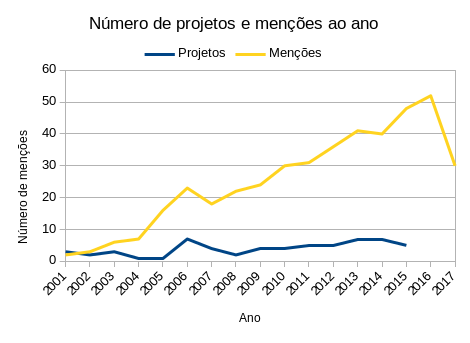
\includegraphics[scale=0.6]{imagens/mentions-projects-by-year.png}
  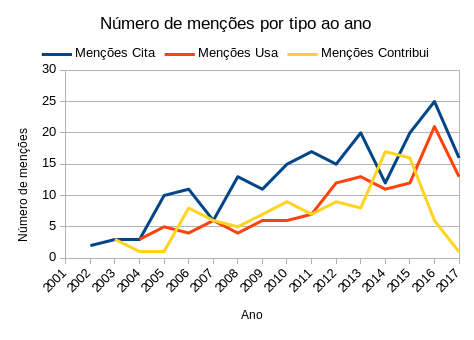
\includegraphics[scale=0.6]{imagens/mentions-type-by-year.png}
  \caption{Número de projetos e menções por tipo ao ano.}
  \label{mentions-by-year}
\end{figure}

Este crescimento, no entanto, pode estar sofrendo influencia do aumento de
projetos, uma vez que há também crescimento no número de projetos a cada ano.
Entretanto, ao isolar os dados, mantendo o número de projetos constante ao longo
do tempo, há um crescimento de 38\% ao ano, conforme Figura
\ref{mentions-trend}.

\begin{figure}[h]
  \center
  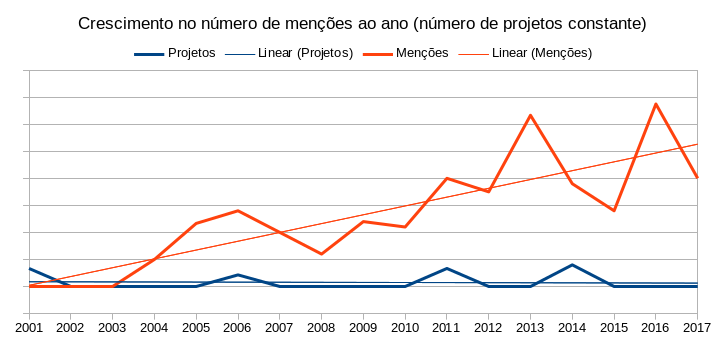
\includegraphics[scale=0.6]{imagens/mentions-trend.png}
  \caption{Crescimento no número de menções ao ano (crescimento médio = 38\%).}
  \label{mentions-trend}
\end{figure}

Entre os 60 projetos de software acadêmico de análise estática estudados, 
13 não possuem reconhecimento acadêmico, ou seja, são
mencionados unicamente no artigo original publicado na ASE ou na SCAM,
que apresentou o software pela primeira vez. 
Os outros 47 projetos possuem maior reconhecimento acadêmico, 
considerando que foram encontradas menções em um ou mais artigos
diferentes da primeira publicação.

%FORA DO ESCOPO: qualidade da citação? 
%FORA DO ESCOPO: como citar software acadêmico?

%Não há relação
%entre as características (número de lançamentos, tamanho em módulos, licença,
%disponibilidade de download, etc) do projetos e o reconhecimento acadêmico.

\subsection{Q2 - \QuestaoDois} % reconhecimento

Há uma evidente relação entre o número de menções e o uso de licenças de
software livre. 
Há 201 menções aos 38 projetos software acadêmico de análise estática sem licença definida, 
enquanto há 228 menções ao 22 projetos com licença, ou seja, 
mesmo com um número menor de projetos, o número de menções encontradas foi 14\% maior, 
conforme Figura \ref{license-vs-mentions}.

\begin{figure}[h]
  \center
  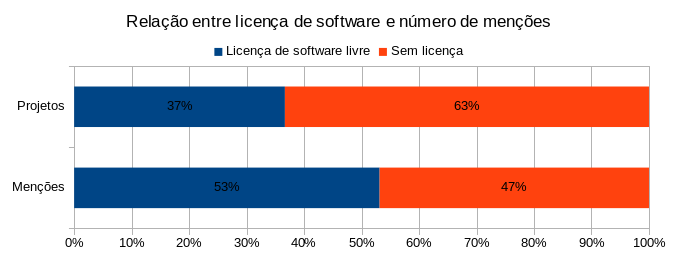
\includegraphics[scale=0.6]{imagens/license-vs-mentions.png}
  \caption{Relação entre o uso de licença de software livre e o número de menções.}
  \label{license-vs-mentions}
\end{figure}

Não foi encontrada relação entre o número de menções e 
outras características do software acadêmico, por exemplo,
disponibilidade para download, linguagem de programação, acesso ao site ou número
de lançamentos.

\subsection{Q3 - \QuestaoTres} % idade média

Os projetos em estágio de {\it Initial development} possuem menos menções em %não deveria haver lançamento, certo?
comparação com o tempo de vida. 
Diferentemente, projetos em estágio de {\it Evolution} ou de {\it Servicing} 
possuem mais lançamentos do que a idade, porém
sendo que o número de menções neste estágio de evolução não é mais disperso. % ou esparso?

A maior parte dos projetos em estágio de {\it Closedown} possui idade superior ao número
de menções, exceto pelos projetos \texttt{s19}, \texttt{s38} e
\texttt{s56} que possuem número de menções bem acima da média geral.
Em especial, o software \texttt{s19} se destaca dentre os projetos com maior número de menções.

Foram encontradas 160 menções para projetos em estágio {\it Closedown}, % Por que acha que isso aconteceu?
71 menções para projetos em estágio de {\it Evolution} ou {\it Servicing} e 
131 menções para projetos em estágio de {\it Initial development}.
%a Figura \ref{mentions-stages-total} detalha estes números.

Os projetos \texttt{s19}, \texttt{s38} e \texttt{s56} são os com maior número de
menções entre os projetos em estágio de {\it Closedown}, com menções
recentes entre os anos de 2017, 2016 e 2014, respectivamente.
% QUAIS OS artigos que os citam? Por que?

\subsection{Q4 - \QuestaoQuatro} % tamanho médio

O tamanho médio do software acadêmico de análise estática publicado nas
conferências ASE e SCAM é de 820 módulos. 
Esta média considera a última versão disponível em código fonte de cada projeto.

%, 22 projetos tiveram seus códigos
%fontes analisados para extrair este dado, os demais projetos não tinham
%código disponível.

O tamanho médio dos projetos em estágio de {\it Initial development} é de 595
módulos. Estes projetos são muito menores que os projetos em estágio de {\it Evolution} 
ou  {\it Servicing} que possuem 1261 módulos, em média. 
Os projetos em estágio de {\it Phaseout} ou {\it Closedown} não possuem código disponível e,
portanto, não sabemos seu tamanho.
A Figura \ref{modules-average} apresenta estes números.

\begin{figure}[h]
  \center
  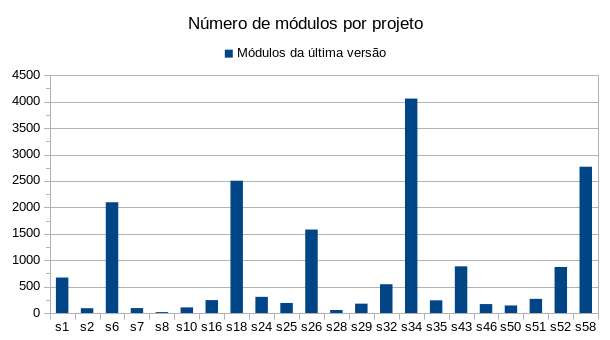
\includegraphics[scale=0.6]{imagens/modules-total.png}
  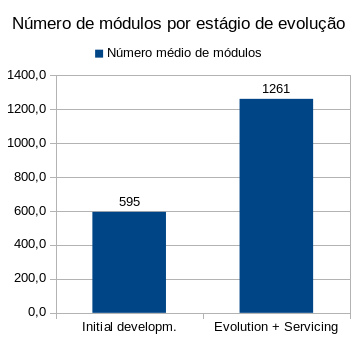
\includegraphics[scale=0.6]{imagens/modules-average.png}
  \caption{Número de módulos por projeto e por estágio de evolução no ciclo de vida.}
  \label{modules-average}
\end{figure}

%(exclui os com valor = 0) são muito menor que osem estágio de evolução e
%serviço  de 1261, ou seja, são pelo menos 2 vezes maior em número de módulos.

De 20 projetos em estágio de {\it Initial development}, 
12 projetos tiveram o código fonte analisado. 
Todos os 8 projetos em estágio de {\it Evolution} ou {\it Servicing}
tiveram seu código fonte analisado.
Vale destacar que estes dois estágios foram agregados num único conjunto 
pois possuem características próximas: 
os 2 projetos em estágio de {\it Evolution} estão
muito mais próximos dos projetos em estágio de {\it Servicing} do que 
do projetos em {\it Initial development}. 

\subsection{Q5 - \QuestaoCinco} % evolução no tamanho

%com reconhecimento
%, entre estes 17 foram
%mencionados em artigos fazendo contribuição, desses 17 10 tem download, 10 tem
%código, 5 initial, 2 servicing, 7 closedown, 3 unknown, 8 tem licença.

Ao analisar a evolução no tamanho (em número de módulos) 
dos projetos em estágio de {\it Servicing}, apresentados na Figura \ref{modules-evolution-servicing},
nota-se um crescimento no número total e médio de módulos
em todos os projetos ao longo dos anos.

%sem reconhecimento
%), entre
%esses 10 tem download, 9 tem código, 5 initial, 2 evolução, 4 closedown, 1
%phaseout, 1 unknown, 3 tem licença.

\begin{figure}[h]
  \center
  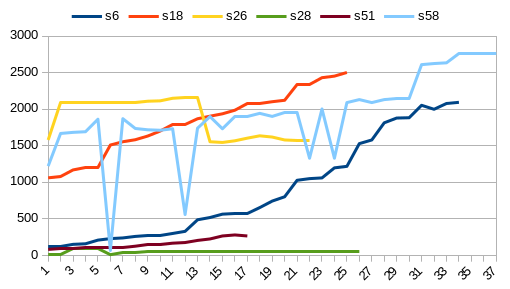
\includegraphics[scale=0.6]{imagens/modules-evolution-servicing.png}
  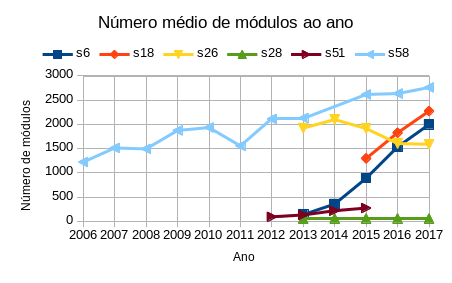
\includegraphics[scale=0.6]{imagens/modules-evolution-average.png}
  \caption{Evolução no número de módulos dos projetos em \textit{Servicing}.}
  \label{modules-evolution-servicing}
\end{figure}

Ao analisar os projetos individualmente, em busca de relação entre
menções e a evolução no tamanho do código fonte (em número de módulos), 
observamos que, para alguns projetos, existe tal relação.
Especulamos que outros projetos podem ter surgido na academia mas 
tiveram seu desenvolvimento posterior externo ao meio científico, 
ao menos para os que foram publicados e indexados nas bases da ACM e do IEEE.

% ACHEI CONFUSO; TENTEI REESCREVER MAS NAO SEI SE FICOU BOM.

\begin{description}

  \item[Software \texttt{s6}.]
    Este projeto teve 5 menções, sendo que em 2015 houve menção do tipo \texttt{Contribui} 
    e em 2017 apenas menções do tipo \texttt{Cita}. 
    Apesar de poucas menções do tipo \texttt{Contribui},
    o projeto apresenta características de estar evoluindo juntamente a atividade
    acadêmica.

  \item[Software \texttt{s18}.]
    Este projeto foi mencionado em apenas 1 artigo em 2012, sendo que o
    primeiro lançamento da versão 2.0 foi em 2015. Este projeto é claramente um
    projeto que ganhou vida própria e seguiu fora da academia.

  \item[Software \texttt{s26}.]
    Este projeto foi mencionado em 7 publicações distintas; em 2014 houve
    menção Contribui, nos anos seguintes possui menções de uso e contribuição.
    A princípio é um projeto com ligação estreita com a atividade acadêmica.

  \item[Software \texttt{s28}.]
    Este projeto está entre os que mais receberam menções, entre 2003 até 2013.
    O projeto tem muitas menções, incluindo contribuições; após 2013, possui apenas
    citações e uso sem novas contribuições. Observa-se uma clara ligação
    entre a evolução do projeto e a atividade acadêmica.

  \item[Software \texttt{s51}.]
    Este projeto teve 4 menções, sendo apenas 1 menção Contribui em 2015,
    e menção Cita e Usa em 2017. O histórico de lançamentos inicia em 2012
    sendo que as primeiras menções aparecem em 2002, o que nos leva a
    questionar: onde estão os lançamentos anteriores a 2012?

  \item[Software \texttt{s58}.]
    Este projeto foi mencionado 11 vezes, sendo apenas 1 menção Contribui em 2010.
    As demais menções são, em grande parte, de uso do software. 
    Entre todos os projetos estudados, este é o que possui maior janela de tempo entre lançamentos, 
    com um histórico de lançamentos de 11 anos. A média dos demais  projetos neste estágio de evolução
    é de apenas 4 anos.

\end{description}

Em resumo, há um crescimento constante no tamanho em número de módulos dos
projetos de software acadêmico de análise estática.
Entretanto, alguns projeto apresentam características de evolução 
totalmente independentes da atividade acadêmica, 
indicando que os seus desenvolvedores, 
apesar de continuar evoluindo os projetos de software,
não tem publicado artigos científicos que os mencionam.

\subsection{Q6 - \QuestaoSeis}

%Entre os projetos em estágio {\it Initial development} apenas 55\% (11) são
%livres -- usam licenças de softawre livre --, entre os projetos em {\it
%Evolution} e {\it Servicing} a maioria 87\% (7) são livres.

Projetos de software acadêmico de análise estática em estágio de {\it Closedown} 
foram encontrados em menções do tipo Usa em 38 artigos 
e em menções do tipo Contribui em 42 artigos.
Estes projetos não estão disponíveis para download, seja binário ou código fonte, 
e a URL indicada pelos autores não permanece acessível, 
indicando que os resultados de tais artigos não podem ser reproduzidos.
%uma vez que acesso aos artefatos do estudo é requisito necessário para esta tarefa.

Em resumo, as pesquisas reportadas em 80 artigos com menção de Uso ou Contribuição em 
software acadêmico de análise estática publicados nas conferências ASE e SCAM 
não podem ser replicadas ou reproduzidas.

%\subsection{Q7 - \QuestaoSete} % é sustentável?

FALAR DE ALGUMA RECOMENDACAO / LICAO? AQUI? NA CONCLUSAO?

ALGUM COMENTARIO SOBRE DCD AQUI? NA CONCLUSAO?



%%---------------------------------------------%%
\section{Recomendações}
\label{sec:recomendacoes}

Os problemas identificados neste estudo podem ser atribuídos em sua maioria a
questões culturais e falta de prática de algumas iniciativas bastante simples
mas muito efetivas para reverter o quadro .... algumas recomendações básicas
pode fazer uma grande diferença neste cenário.

Recomendações aos desenvolvedores de software acadêmico:

\begin{itemize}
  \item Sempre publicar o código fonte do software acadêmico!
  \item Utilizar licenças de software livre, especialmente licenças com mecanismo de copyleft, exemplo: GPL.
  \item Publicar o software em fontes com maior garantia de longevidade, como por exemplo, Github, Gitlab, Savannah ou Sourceforge
  \item Evitar publicar o software em infraestrutura particular ou própria, como por exemplo os servidores da universidade, tendem a mudar de endereço ou serem descontinuados.
  \item Fornecer instrução sobre como citar o software adequadamente, se possível incluir no repositório do projeto um arquvo BibTeX \texttt{paper.bib} com os metadados de como deve ser citado.
  \item Quando possível, dar preferência a colaborar com projetos existentes em detrimento de iniciar e desenvolver novos
  \item Publicar o software em jornais específicos para software e ferramentas, exemplos: JOSS, JORS e SoftwareX.
\end{itemize}

Recomendações aos usuários de software acadêmico:

\begin{itemize}
  \item Sempre indicar a versão do software utilizado na pesquisa.
  \item Quando possível fazer uso de citação formal ao mencionar software acadêmico, verique se o software fornece sugestão de como ser citado.
%  \item ao implementar provas de conceitos de novos algoritmos em estudos avaliando e comparando ferramentas enviar quando possível contribuição aos projetos utilizados
%* evitar manter guardado qualquer código implementado, mesmo que pareça inicialmente não útil para outros
\end{itemize}

Lições, a revisão de literatura realizada para encontrar menções a software
representa um alto grau de dificuldade e trabalho ``braçal'' uma vez que uma
revisão deste tipo seria simplificada muitissimo caso o software fosse citado
através de citação formal, uma vez que desta forma existem inúmeras soluções para
busca, metadados, ligações entre a literatura, etc... mas o fato de não haver
prática padronizada sobre como citar software, descobrir na literatura quando
umm software é citado é um trabalho de certa forma desencorajador, ...

%entre os projetos usando licenças de software livre há um maior número de menções (14\% mais menções que os demais projetos
%FALAR DE DCD aqui? ver últimas frases do RESUMO.

%O ecossistema de software, assim como nos sistemas naturais, necessita de
%fornecimento constante de energia para se manter estável e sustentável, notamos
%no entando que o ecossistema de software acadêmico de análise estática carece
%de investimento, especialmente em termos de contribuição de código fonte, onde


%O desenvolvimento de software sustentável tem sido identificado como um desafio chave no
%campo da Ciência e da Engenharia Computacional. Se sustentabilidade não for levada em
%consideração em projetos de software, não importa qual o domı́nio ou qual o propósito do
%software, perde-se a oportunidade de causar mudanças positivas no planeta e na sociedade
%(BECKER et al., 2014).

%, não sabemos no entanto qual a relação de causa e
%efeito em relação a este maior número de menções aos projetos usando licenças
%livres.

%Alguns projetos de software acadêmico evoluem de maneira independente
%de qualquer atividade acadêmica, com atualizações constantes e lançamentos de
%novas versões ao longo do tempo mas sem nenhuma menção recente na literatura
%acadêmica a respeito do software, 78\% dos projetos estão em estágio inicial de
%desenvolvimento ({\it Initial development}), encerrados ({\it Closedown}) ou
%sendo encerrados ({\it Phaseout}), apenas 13\% dos projetos estão em evolução
%({\it Evolution}) ou provendo serviços ({\it Servicing}).
%
%O tamanho médio do software acadêmico de análise estática em termos de número
%de módulos em estágio {\it Evolution} e {\it Servicing} é duas vezes maior que
%os projetos em {\it Initial development}, a evolução dos projetos mostra um crescimento
%constante no número de módulos no código fonte, confirmando a lei de Lehman de ``Crescimento Contínuo'' do software
%\cite{lehman1997metrics}.

%constantes. Sendo considerados como bons candidados a projetos úteis para uso
%em outras pesquisas.

%%%%%%%%%%%%%%%%%%%%%%%%%%%%%%%%%%%%%%%%%%%%%%%%%%%%

%... 19\%, ou seja, 80 artigos mencionando Uso ou Contribuição a software
%acadêmico de análise estática publicados nas conferências ASE e SCAM não podem
%ser replicados ou reproduzidos.

%apresentam características
%de terem sido desenvolvidos sem preocupação com a sustentabilidade técnica

%mantidos de forma tecnicamente sustentável, ou seja, não são disponíveis para
%obtenção, estão em estágio inicial de desenvolviment ou foram encerrados.

%Observamos que 78\% dos projetos de software acadêmico de análise estática
%encontram-se em estágio inicial de desenvolvimento ({\it Initial development})
%sendo encerrados ({\it Phaseout}) ou já encerrados ({\it Closedown}). Indicando
%que temos neste domínio muitos projetos sem atividade de evolução após a sua
%criação e publicação.

%9\% não foram caracterizados em termos de ciclo de vida por falta de informaçao e 

%Os projetos em estágio inicial apesar de não serem considerados projetos em
%estágio de serem utilizados em outras pesquisa são bons candidados a serem
%adotado em outras pesquisa como ponto de partida inicial para a adaptação e
%atender novas demandas.

%O código fonte de 206 versões foram analisados e os projetos foram
%caracterizados em estágios de evolução, entre {\it Initial development}, {\it
%Evolution}, {\it Servicing}, {\it Phaseout} ou {\it Closedown}.

%, este
%crescimento reflete o papel cada vez maior que o software possui na Ciência,
%mas apesar disso há ainda uma porção de software sem qualquer reconhecimento na
%literatura acadêmica, 21\% dos projetos não possuem qualquer menção além do
%artigo inicial onde foram publicados originalmente, 43\% dos projetos são
%utilizados em artigos além da publicação inicial e apenas 28\% recebem
%contribuição em código fonte.

%Uma avaliação sobre o nível de reconhecimento a estes projetos em publicações
%nas bases da ACM e IEEE encontrou 416 artigos mencionando os projetos de
%software acadêmico, entre 199 menções do tipo Cita, 124 do tipo Usa e 106 do
%tipo Contribui.

%Este uso é mencionado na literatura academica por meio de citação formal ou in-
%formal (SMITH; KATZ; NIEMEYER, 2016) e está estreitamente relacionado ao sistema
%econômico de reputação cientı́fica, uma vez que menções causam impacto cientı́fico direto
%tanto na publicação quanto no ecossistema de software acadêmico (KATZ, 2014).
%Este impacto direto geralmente justifica o investimentos de novos recursos no ecos-
%sistema, seja para fins de planejamento, por exemplo, uma retrospectiva para avaliar
%investimentos já realizados ou para fins de promoção e evolução do software acadêmico
%(HOWISON et al., 2015).

%com a identificação
%do nome do projeto e endereço URL para download do software, 60\% dos projetos
%de software acadêmico publicados nestes artigos encontram-se disponíveis para
%download, apenas 56\% possuem código fonte disponível publicamente, 35\%
%utilizam licenças de software livre.

%Esses artigos publicam 60 projetos de software acadêmico de
%análise estática, dentre os quais, 

%Entre 1873 artigos publicados nas conferências de Engenharia de Software ASE e
%SCAM até o ano de 2015 apenas 61 artigos publicam software acadêmico de análise
%estática publicizados minimamente com identificação do nome do projeto e URL
%para obtenção.


\section{Trabalhos relacionados}
\label{sec:trabalhosrelacionados}

\citeonline{segal2008developing}
investigam como o desenvolvimento de software acadêmico pode ser melhorado e
enfatiza as diferenças do software acadêmico em relação aos demais tipos de
software, onde o conhecimento sobre o domínio pode muitas vezes incluir temas
avançados e pouco comuns fora do meio científico.

\citeonline{knutson2010report}
ao resumir as conclusões do evento RESER (Workshop on Replication in Empirical
Software Engineering Research) de 2011 cita que ferramentas de software
acadêmico estão indisponíveis ou não são usáveis em estágios não útil, tornando
replicação precisa impraticável.

\citeonline{robles2010replicating} num revisão de 171 artigos do MSR entre 2004 e 2009
em busca de conjunto de dados, artefatos e ferramentas utilizadas nos estudos
necessárias para replicação mostrou que a maioria dos artigos não conseguiram encontrar
as ferramentas mesmo quando o autor explicitamente afirma que fizeram uma.

%\citeonline{holcombe2011openaccess} no projeto {\it Open Access Pledge}
%\footnote{\url{http://www.openaccesspledge.com}} concentra-se em publicar
%softwares e papers em locais de {\it open access}.

\citeonline{portillo2012tools}
através de um mapeamento sistemático mostra que grande parte das ferramentas de
software criadas na academia estão em estado inicial de desenvolvimento que
apenas uma pequena porcentagem são testados fora do contexto onde foi
desenvolvido. 

\citeonline{chaturvedi2013tools}
faz uma revisão de literatura entre artigos submetidos ao MSR de 2007 até 2013,
identifica conjunto de dados, ferramentas e técnicas utilizadas pelos autores,
mais da metade dos artigos usam ou criam ferramentas, categoriza as ferramentas
em ferramentas novas, ferramentas tradicionais, protótipos e scripts para
mineração de dados.

\citeonline{barnes2013science}
cria o manifesto {\it Science Code Manifesto} e enfatiza que todo código fonte
escrito especificamente para processar dados de publicações devem estar
disponíveis aos revisores e leitores do paper.

\citeonline{marshall2013tools} num mapeamento sistemático sobre artigos criando
ferramentas de apoio a revisão sistemática no domínio de SE conclui que as
ferramentas encontradas estão em estado inicial de desenvolvimento.

\citeonline{hettrick2014uk} mostra que no reino unido entre todas as áreas da
ciência 56\% dos cientistas estão envolvidos no desenvolvimento de software
acadêmico.

\citeonline{wilson2014best} resume as melhores práticas para melhoria da
manutenibilidade e disponibilidade do software acadêmico desenvolvido por
cientistas.

\citeonline{wilson2014software} num resumo sobre as lições aprendidas em 20
anos da iniciativa {\it Software Carpentry} sobre atividades de melhoria das
habilidades dos pesquisadores com computacao.

\citeonline{amann2015software}
investigam através de uma revisão sistemática de literatura uma década de
publicações e encontram que muito poucos estudos são replicáveis visto que
faltam informações incluindo dados e ferramentas, apenas 20\% dos estudos
possuem ferramentas disponíveis.

\citeonline{momcheva2015software}
num survey com 1142 participantes sobre o uso de software em pesquisas da
astronomia mostrou que 90\% dos cientistas escrevem software e 100\% usam
software em suas pesquisas.

\citeonline{beller2016analyzing} avalia e sugere caminhos para melhorar o
desenvolvimento de ferramentas de análise estática com o objetivo de aumentar a
adoção.

\citeonline{smith2016software} resume recomendações sobre como citar software
na literatura acadêmica com objetivo de encorajar uma ampla adoção e uma
política consistente para citação de software entre as múltiplas disciplinas.

\citeonline{smith2016software} afirma que ``citações aos softwares devem
permitir e facilitar acesso ao software, metadados, documentação, dados e
outros materiais necessários tanto para humanos quanto para máquinas''.

%\citeonline{wilkinson2016fair} através do {\it FAIR
%principles}\footnote{\url{https://www.nature.com/articles/sdata201618}} com
%foco em dados de pesquisa, o objetivo é fazer eles serem encontráveis,
%acessíveis, interoperável e reusável. Estes princípios podem ser generalizados
%para aplicar aos softwares.

\citeonline{howison2016software}
numa revisão de literatura mostrou que publicações usando softwares como
método, mostrou que apenas 59 mencionavam o uso de softwares de alguma forma,
os demais 31 artigos, apesar de usar software acadêmico, não mencionavam nada a
respeito.

\citeonline{wilson2017good} apresenta um conjunto de boas práticas que todo
pesquisador pode adotar, independentemente do seu nível de habilidade em
computação. Essas práticas passam por gerenciamento de dados, programação,
colaboração com colegas, organização de projetos, tracking work, e escrita da
manuscritos.
%, sao desenhados para uma grande variadade de fontes publicadas do
%noso dia a dia e do nosso trabalho como voluntário organizando workshopts desde
%2010.

%Open Science Peer Review Oath\footnote{\url{https://f1000research.com/articles/3-271/v2}}
%Concentra-se em potencializar os revisores para exigir acesso aberto aos
%softwares, práticas reprodutíveis e revisões transparentes.

%Muitos pesquisadores não
%disponibilizam os seus softwares
 %ou quanto o fazem enfrentam problemas com disponibilidade e
%manutenibilidade \cite{prlic2012ten}

%Entretanto, ao analisar o crescimento no número de menções isolando a influência do
%crescimento no número de projetos nota-se que a taxa de crescimento isolada do
%crescimento de projetos, o número de menções cresce numa taxa de

%... a Figura \ref{mentions-by-year} (a) é possível notar uma clara relação
%entre o número total de menções e o número de projetos novos por ano, ou seja,
%ao subir o número de projetos sobe também, numa proporção muito maior, o número
%de menções. Quanto mais projetos mais menções, mas também o número de menções
%a software de modo geral cresce ...

%... a Figura \ref{mentions-by-year} (b) apresenta o número de menções por tipo Cita, Usa e Contribui ao
%ano onde é possível notar que ambos os tipos apresentam crescimento similar ao longos dos anos ...

%Esta análise para simular um número constante de projetos publicados ao ano foi
%realizada selecionando o número de menções ao ano para um conjunto de no máximo
%3 projetos selecionados aleatoriamente, visto que o número de projetos em
%alguns anos não chega a 3, e para alguns projetos o número de menções é muito
%baixa, repetimos esta seleção algumas vezes até obter um número desejável e
%calculamos a média do número de menções em cada ano.

%, utilizamos várias amostras de menções por
%ano capturando grupos distintos de no máximo 3 projetos e as menções a estes projetos,
%a taxa de crescimento média de menções ao longo dos anos é de 38\%, ou seja,
%permanecendo constante o número de projetos ao ano, as menções irão crescer numa taxa
%de 38\% ao ano na média ...

%Uma questão interessante é a de ``integridade''. 
%O que acontece com os resultados anteriores (publicados)
%se houver um erro ou uma mudança substancial da forma de calcular algo?
%Na prática, só deveríamos permitir refactorings no código 
%de um software acadêmico ou adição de novas funcionalidades?
%(Chris)
%
%An so what?
%
%O ecossistema de software acadêmico de análise estática sofre de disfunctional ...?

%Encarar o software acadêmico como a "plataforma" do ecossistema de software.
%Pensar no ecossistema de pesquisa e produção intelectual.

%Não encontramos relação entre disponibilidade de download e menções, seja Cita, Usa ou Contribui.


%O número de menções encontradas de cada projeto não sofre influência de suas
%características de publicização ou
%No entando
%
%  13 projetos foram encontrados num único e mesmo artigo já encontrado no estudo anterior
%    (s1, s13, s17, s20, s21, s24, s35, s41, s42, s43, s47, s50, s55)
%  47 foram encontrados em menções
%    17 recebem contribuições
%      (s4, s5, s8, s9, s10, s19, s23, s25, s26, s28, s32, s37, s40, s45, s49, s52, s59)

%A idade média do software acadêmico de análise estática publicado nas
%conferências ASE e SCAM é de 7,6 anos. Foi considerado como ano de nascimento
%de cada projeto a data do primeiro lançamento ou da primeira menção ao projeto.
%Com isso calculou-se a idade com base no ano de 2017, ou seja, subtraimos 2017
%do ano de nascimento.

%Ao por em contraste a idade de cada projeto com o número de lançamentos e o
%número de menções, conforme Figura \ref{age-releases-mentions}, percebe-se que

%a idade dos projetos em {\it Initial development} é superior ao número de
%lançamentos, na maior parte é também superior que o número de menções, 

%\begin{figure}[h]
%  \centering
%  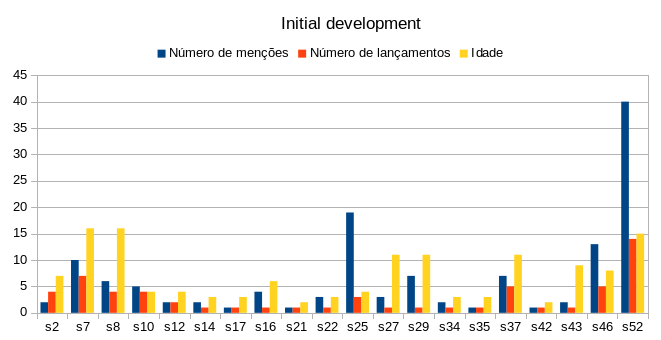
\includegraphics[scale=0.6]{imagens/age-initial-development.png}
%  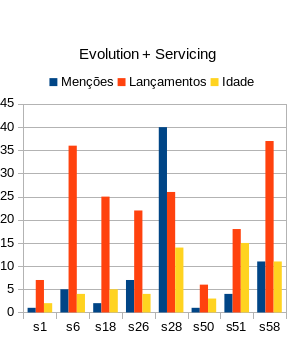
\includegraphics[scale=0.6]{imagens/age-evolution-servicing.png}
%  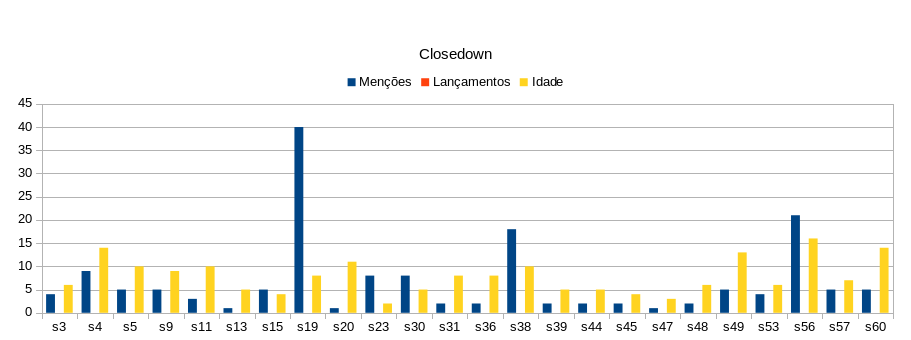
\includegraphics[scale=0.6]{imagens/age-closedown.png}
%  \caption{Número de menções, lançamentos e idade de cada projeto por estágio de evoluçao.}
%  \label{age-releases-mentions}
%\end{figure}

%de menções entre os similar aos dois outros projetos mas que encontram-se em
%initial ou evolution e estão disponiveis para download, inclusive em código
%fonte. Algp que este projeto \texttt{s19} não reflete.

%A idade de cada projeto foi calculada
%considerados todos os anos em que houve lançamento
%ou foram encontradas menções ao software,
%entre todo o período encontrado para cada software, o primeiro ano onde uma
%das ocorrências tenham acontecido, aquela mais antiga, foi considerada como
%Idade VS lançamentos VS menções dos projetos em initial development.
%Idade VS lançamentos VS menções dos projetos em Evolution e Servicing.

%Initial tem idade minima 2 (todos tem essa idade minima ja que a data limite na selecao foi 2015)

%A média de idade entre os estágios de evolução é aproximadamente igual, {\it
%Evoution} com média 7,3, {\it Initial development} 7,1 e {\it Closedown} 7,9.
%A média de idade entre os projetos disponível para download e não disponíveis
%para download é o mesmo, 7. Os projetos em estágio {\it Servicing} possuem
%entre 4 e 15 anos de idade. A idade mínima de todos os projetos é 2 anos, já
%que a revisão de literatura para seleção dos projetos limitou-se ao ano de
%2015.

%Mas ao considerar apenas os períodos com lançamentos ou menções, os projetos em
%{\it Evolution} e {\it Servicing} tem média superior
%
%Mas o delta entre a última ocorrencia (release ou mencao) e a primeira é maior,
%nos projetos em servicing e evolution = 7.3,
%enquanto no initial = 4.8 e close = 4.9. Ou seja, se considerarmos a mesma data de nascimento
%mas usar a data final contando a última ocorrência encontrada, seja entre as menções, seja
%entre os lançamentos, os projetos em Servicing e Evolution apresentam um intervalo maior. Isto
%representa que estes projetos tem uma janela de atividade (seja acadêmica, seja fora dela) maior que
%os projetos em Closedown e Initial development.
%
%Importante lembrar que a própria caracterização em relação ao estágio utilizou
%as atividades de lançamento como ponto de partida, não foi o único critério, nem o mais
%definitivo, mas os projetos que tiveram somente uma ocorrência de lançamento ou de menção por exemplo
%foram todos classificados como initial.

%, ou seja, não há entre
%os projetos software mais recente do que 2015.

%\begin{figure}[h]
%  \center
%  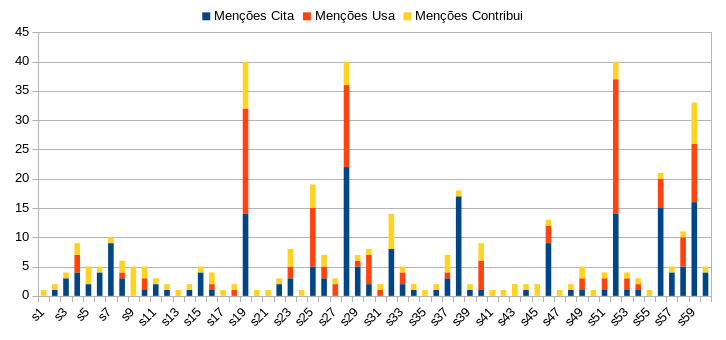
\includegraphics[scale=0.6]{imagens/mentions-by-type.png}
%  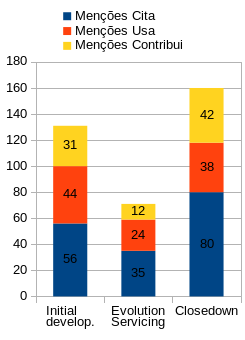
\includegraphics[scale=0.6]{imagens/mentions-stages-total.png}
%  \caption{Número total de menções por tipo.}
%  \label{mentions-stages-total}
%\end{figure}

%... a Figura \ref{mentions-stages-total} ... 

%      37 sem licença =       200 menções
%-38\% 23 com licença = +14\% 229 menções
%
%      24 sem download =       160 menções
%+50\% 36 com download = +68\% 269 menções
%
%19 projetos acima de 1 menção Contribui
%  260 menções ao total
%  184 lançamentos, 
%  7 closedown, 7 initial, 2 servicing
%
%39 projetos até 1 menção Contribui
%  169 menções
%  119 lançamentos
%  19 closedown, 2 evolution, 13 initial, 1 phaseout, 4 servicing

%1873 (ASE e SCAM) artigos encontrou 60 projetos
%  24 (40\%) não estão disponíveis para download
%  36 (60\%) estão disponíveis para download
%    34 estão disponíveis em código fonte
%      13 não declaram licença
%      21 usam licenças FOSS
%    2 estão disponíveis apenas em binário
%
%busca pelos 60 projetos encontrou 806 artigos (ACM e IEEE)
%  429 menções em 416 artigos
%    199 cita
%    124 usa
%    106 contribui

%\begin{figure}[h]
%  \center
%  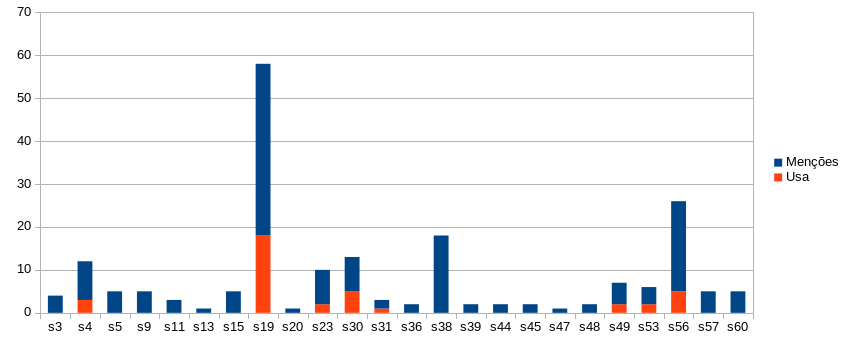
\includegraphics[scale=0.6]{imagens/closedown-mentions-vs-use.png}
%  \caption{Número total de menções em relaçao a menções do tipo {\it Usa} entre os projetos em estágio {\it Closedown}.}
%  \label{closedown-mentions-vs-use}
%\end{figure}

%Média de menções por grupo de estágio de evolução.
%
%\begin{figure}[ht]
%  \begin{minipage}{0.32\textwidth}
%    \centering
%    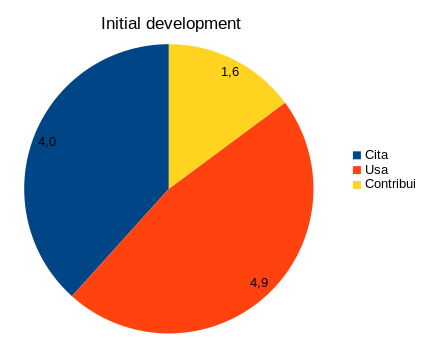
\includegraphics[scale=0.5]{imagens/mentions-initial-development.png}
%  \end{minipage}
%  \begin{minipage}{0.32\textwidth}
%    \centering
%    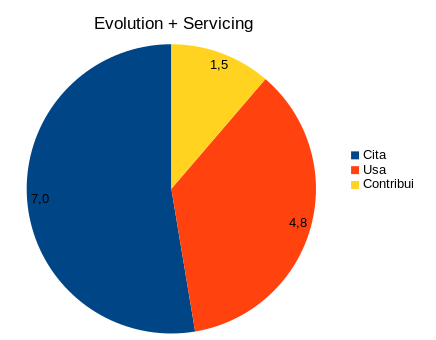
\includegraphics[scale=0.5]{imagens/mentions-evolution-servicing.png}
%  \end{minipage}
%  \begin{minipage}{0.32\textwidth}
%    \centering
%    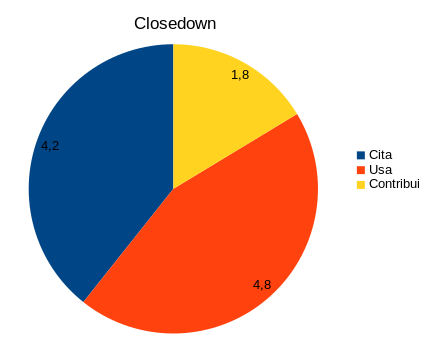
\includegraphics[scale=0.5]{imagens/mentions-closedown.png}
%  \end{minipage}
%  \caption{...}
%  \label{mentions-stages-blah}
%\end{figure}

